% Projeto de Conclusão de Curso
% Aluno: xpto
%----------------------------
\documentclass[
	12pt,	
    oneside,
    a4paper,
    brazil  
]{abntex2}

% ----------------------------
% Pacotes para acentuação
% ----------------------------
    \usepackage[T1]{fontenc}
    \usepackage{lmodern}
    \usepackage{sty/sbc-template}
    \usepackage[utf8]{inputenc}
    \usepackage{adjustbox}    % Escala/resize
    \usepackage{longtable}    % Multi-página
    \usepackage{rotating}     % Paisagem
    \usepackage{booktabs}

%--------------------------------------------
% Variáveis para preencher com os seus dados
%--------------------------------------------
    \title{Lógica computacional como estrutura intermediária para tradução entre representações}
    \subtitle{Uma proposta para tradução bidirecional entre código e blueprints visuais}
    \author{Anna Beatriz Resende Oki Corrêa}
    \cidade{Brasília}
    \ano{2026}
    \coordenacao{Coordenação do Curso de Sistema de Informações}
    \titulacao{ Sistema de Informações}
    \orientador{Prof. Dr. Xxxx}
%--------------------------------------------


\renewcommand{\listfigurename}{}
\begin{document} 
\pagestyle{empty}
\maketitle
\newpage


% -------------------------------
% Registro Bibliográfico
% Faça as modificações nos campos que estão indicados com ??
% -------------------------------
\section*{}
\vspace*{80pt}
\begin{center}
\begin{tcolorbox}[
    enhanced, % Permite a personalização avançada
    sharp corners, % Torna os cantos afiados
    width=1.0\textwidth, % Largura da caixa
    colback=white, % Cor de fundo
    colframe=black, % Cor da primeira borda
    boxrule=3pt, % Largura da primeira borda
    boxsep=20pt, % Espaçamento entre o texto e as bordas
    frame style={draw=black, double distance=4pt, double, ultra thick}, % Estilo da segunda borda
    ]
    ?Sobrenome?, ?Nome?. 
    \hspace{1cm} Título : \titulo / ?author?. -- Brasília, 2026. 
    \hspace{1cm} \pageref{LastPage} f. \\[2mm]
   	Orientador: ?orientador?. 
    \hspace{1cm}Trabalho de Conclusão de Curso (Graduação -- Sistema de Informações) -- Centro Universitário do Distrito Federal -- UDF. Coordenação do Curso de Sistema de Informações, Brasília, DF, 2026. \\[2mm]
   	1. ?Assunto?. 2. ?Assunto?. 3. ?Assunto?. I. ?Título?. \\[2mm]
   	\begin{flushright}
    CDU: ?consultar na biblioteca?
    \end{flushright}
\end{tcolorbox}
\end{center}


% -------------------------------
% Assinaturas
% Faça as modificações nos campos que estão indicados com ??
% -------------------------------
\newpage
\section*{}

\vspace*{10pt}
\begin{center}
?Titulo?
\vspace*{60pt}
\begin{adjustwidth}{6cm}{-1cm}
Trabalho de conclusão de curso apresentado à ?Coordenação?, do Centro Universitário do Distrito Federal -- UDF, como requisito parcial para obtenção do grau de bacharel / tecnólogo em ?Curso?. \\[2mm]

Orientador: ?orientador?. 
\end{adjustwidth}
\vspace*{40pt}
Brasília, \underline{\hspace{2cm}} de \underline{\hspace{4cm}} de 2026.

\vspace*{60pt}
\begin{tabular}{p{7cm}}
    \hline
    \centering NOME DO EXAMINADOR \\
    \centering Titulação \\
    \centering Instituição a qual é filiado
\end{tabular}

\vspace*{30pt}
\begin{tabular}{p{7cm}}
    \hline
    \centering NOME DO EXAMINADOR \\
    \centering Titulação \\
    \centering Instituição a qual é filiado
\end{tabular}

\vspace*{30pt}
\begin{tabular}{p{7cm}}
    \hline
    \centering NOME DO EXAMINADOR \\
    \centering Titulação \\
    \centering Instituição a qual é filiado
\end{tabular}
\end{center}

\vspace*{40pt}
Nota: \underline{\hspace{2cm}}


% -------------------------------
% Dedicatórias
% -------------------------------
\newpage
\begin{dedicatoria2}{}
 Dedico este trabalho à minha família, pelo apoio, incentivo e compreensão durante toda a minha trajetória acadêmica.
 \end{dedicatoria2}

% -------------------------------
% Agradecimentos
% -------------------------------
\newpage
\begin{agradecimento}{Agradecimentos}
Agradeço, primeiramente, a Deus, por mais uma conquista; ao meu orientador, pela dedicação e correções; e aos bibliotecários pelo suporte em todas as pesquisas.

\end{agradecimento}


% -------------------------------
% Frase motivacional
% -------------------------------
\newpage
\begin{adjustwidth}{7cm}{0cm}
\vspace*{\fill}
\begin{flushright}
"A educação é a arma mais poderosa que você pode usar para mudar o mundo." \\
\vspace*{10pt}
Nelson Mandela
\end{flushright}
\end{adjustwidth}


% -------------------------------
% Resumo
% -------------------------------
\newpage
\begin{resumo2}
Este trabalho investiga a relação existente entre diferentes formas de representação computacional, considerando linguagens de programação textuais, fluxogramas, sistemas baseados em nós (blueprints) e plataformas Low-Code e No-Code. A pesquisa parte da hipótese de que essas representações, apesar de apresentarem características visuais e sintáticas distintas, compartilham uma mesma estrutura lógica subjacente. Por meio de revisão bibliográfica e análise conceitual, discute-se o papel da abstração na computação e a possibilidade de separar a lógica computacional de sua forma de representação. Como resultado, é proposto um modelo conceitual no qual uma estrutura lógica intermediária atua como elemento de integração entre diferentes representações computacionais, permitindo compreender como um mesmo algoritmo pode ser expresso por mecanismos distintos sem alteração de seu comportamento fundamental. A proposta busca contribuir para discussões relacionadas à interoperabilidade entre ambientes de desenvolvimento e à tradução entre representações computacionais.

\vspace*{20pt}
\textbf{Palavras-chave:}lógica computacional; programação visual; blueprints; low-code; representação computacional.
\end{resumo2}


% -------------------------------
% Abstract - Resumo traduzido para o Inglês
% -------------------------------
\newpage
\begin{abstract}
This research investigates the relationship between different forms of computational representation, including textual programming languages, flowcharts, node-based systems (blueprints), and Low-Code and No-Code platforms. The study is based on the hypothesis that, despite their visual and syntactic differences, these representations share a common underlying logical structure. Through a literature review and conceptual analysis, the research discusses the role of abstraction in computing and the possibility of separating computational logic from its representation form. As a result, a conceptual model is proposed in which an intermediate logical structure acts as an integration element between different computational representations, enabling the understanding of how the same algorithm can be expressed through distinct mechanisms without changing its fundamental behavior. The proposal aims to contribute to discussions related to interoperability between development environments and the translation between computational representations.

\vspace*{20pt}
\textbf{Keywords:} computational logic; visual programming; blueprints; low-code; computational representation.
\end{abstract}


% -------------------------------
% Lista de Figuras
% -------------------------------
\newpage
\listoffigures*

% -------------------------------
% Lista de Tabelas
% -------------------------------

% -------------------------------
% Lista de Abreviaturas e Siglas
% -------------------------------
% No documento use: Isso é um \ac{ex}.
% --------------------------------
\chapter*{Siglas}
\begin{acronym}
\acro{IA}{Inteligência Artificial}
\acro{UML}{Unified Modeling Language}

\end{acronym}

\clearpage


% -------------------------------
% Sumario
% -------------------------------
\tableofcontents*
%\cleardoublepage

 
% -------------------------------
% INICIO DO TRABALHO - CAPÍTULOS
% -------------------------------
\textual 
\chapter{Introdução}
A lógica computacional constitui um dos elementos fundamentais do desenvolvimento de software, estando relacionada à definição de regras, decisões, condições, operações e fluxos que determinam o comportamento de um sistema. A construção de um programa envolve, portanto, a organização desses elementos de maneira que possam ser interpretados e executados por um sistema computacional. Entretanto, a compreensão de um programa não depende exclusivamente da forma concreta em que suas instruções são escritas, uma vez que os elementos lógicos podem ser analisados em diferentes níveis de abstração.

A abstração constitui um mecanismo fundamental para lidar com a complexidade presente na computação. Por meio dela, características específicas de uma implementação podem ser ocultadas para que sejam considerados os elementos relevantes de um determinado problema. \citeonline{abelson1996} apresentam a abstração como um mecanismo importante para organizar sistemas computacionais e trabalhar com diferentes níveis de representação. Dessa forma, uma mesma estrutura computacional pode ser analisada considerando seus elementos fundamentais sem que seja necessário restringir sua compreensão a uma implementação específica. Essa perspectiva permite distinguir a lógica de um programa da forma utilizada para expressá-la.

A partir dessa possibilidade de abstração, diferentes formas de programação e representação foram desenvolvidas ao longo da evolução da computação. As linguagens de programação textuais expressam estruturas computacionais por meio de instruções e elementos sintáticos, enquanto abordagens visuais utilizam elementos gráficos para organizar e construir programas. Entre essas abordagens encontram-se linguagens baseadas em blocos, sistemas baseados em nós e outras formas de programação visual. \citeonline{myers1990} apresenta uma taxonomia das linguagens de programação visual, discutindo diferentes formas de utilizar representações gráficas como parte do processo de programação. O autor também diferencia programação visual de técnicas destinadas apenas à visualização de programas, distinção importante para esta pesquisa.

A programação visual, portanto, não deve ser compreendida simplesmente como uma representação gráfica de um código textual já existente. Em determinadas abordagens, os próprios elementos visuais constituem os mecanismos utilizados para construir a lógica do programa. Blocos, nós, conexões e outros componentes gráficos podem representar operações, relações, condições e fluxos, permitindo que o programa seja construído por meio dessas estruturas. Essa característica faz com que diferentes ambientes visuais possam apresentar formas distintas de organizar uma mesma classe de elementos computacionais.

A relação entre programação visual e programação textual também é discutida na literatura sob diferentes perspectivas. \citeonline{noone2018} realizaram uma revisão sistemática da literatura sobre linguagens de programação visuais e textuais, investigando principalmente seu papel no processo de aprendizagem de programação. A revisão reúne estudos que discutem as características e o uso dessas duas formas de programação, evidenciando que a relação entre representações visuais e textuais constitui um tema de investigação dentro da área de ensino de programação.

Além da revisão da literatura, existem estudos empíricos que analisam a utilização de ambientes visuais em situações concretas de aprendizagem. \citeonline{saezlopez2016} realizaram um estudo de dois anos em cinco escolas, envolvendo 107 estudantes, utilizando o Scratch como ambiente de programação visual. Por meio de uma abordagem quase-experimental, os autores observaram resultados relacionados à aprendizagem de conceitos de programação, lógica e práticas computacionais. Esses resultados fornecem evidência empírica sobre o uso de programação visual em um contexto educacional específico, mas não permitem afirmar que a programação visual seja universalmente superior à programação textual.

A combinação dessas perspectivas permite observar que a programação visual pode ser analisada tanto conceitualmente quanto empiricamente. \citeonline{myers1990} fornece uma base para compreender o que caracteriza uma representação visual utilizada na programação; \citeonline{noone2018} apresentam uma visão sistematizada da literatura sobre linguagens visuais e textuais; e \citeonline{saezlopez2016} apresentam evidências obtidas a partir da aplicação de um ambiente visual em um contexto educacional. Essas diferentes abordagens são relevantes para compreender que as formas de programação podem utilizar mecanismos de representação distintos, ainda que trabalhem com conceitos computacionais relacionados.

Nesse contexto, uma mesma estrutura lógica pode assumir diferentes formas de expressão. Uma condição, por exemplo, pode ser escrita por meio de uma estrutura textual, organizada por blocos ou representada por nós conectados em um fluxo. A alteração da representação não implica necessariamente uma alteração no comportamento lógico pretendido. Para esta pesquisa, essa distinção é fundamental, pois permite analisar separadamente a estrutura lógica de um programa e a forma utilizada para expressá-la.

Dessa perspectiva, este trabalho estabelece uma distinção entre lógica computacional e representação computacional. A lógica computacional corresponde ao conjunto de regras, operações, decisões e relações que determinam determinado comportamento, enquanto a representação computacional corresponde ao mecanismo utilizado para expressar esses elementos. Código textual, blocos e grafos de nós podem, portanto, constituir diferentes formas de representação de estruturas lógicas computacionais.

Entre as diferentes formas de programação visual, os sistemas baseados em nós constituem um caso particularmente relevante para esta investigação. Nesses ambientes, elementos gráficos são conectados para representar operações, eventos, condições e fluxos de execução. Um exemplo é o sistema de \textit{Blueprint Visual Scripting} da Unreal Engine, descrito por \citeonline{romero2014blueprint} como uma linguagem visual de programação baseada em nós. Nesse contexto, os \textit{Blueprints} constituem um exemplo concreto de como estruturas lógicas podem ser representadas visualmente e executadas em um ambiente computacional.

A existência de diferentes representações conduz a uma questão relacionada à comunicação e transformação entre essas formas. Quando uma lógica construída em uma determinada representação precisa ser expressa em outra, não basta necessariamente reproduzir seus elementos visuais ou sintáticos. É necessário identificar as estruturas e relações que determinam seu comportamento e preservá-las durante a transformação. Surge, assim, o problema de investigar como diferentes representações podem estabelecer correspondências entre si sem perder os elementos fundamentais da lógica computacional.

Nesse cenário, a Inteligência Artificial apresenta uma possibilidade de apoio à interpretação e transformação dessas representações. Modelos capazes de processar linguagem e estruturas de código podem receber uma representação de origem, interpretar seus elementos e produzir uma representação em outro formato. Entretanto, é necessário investigar em que medida esses modelos conseguem preservar a lógica presente na representação original e quais mecanismos podem contribuir para essa preservação.

Uma possibilidade considerada neste trabalho é a utilização de uma representação lógica intermediária, capaz de organizar os elementos comuns entre diferentes formas de programação. Essa estrutura poderia funcionar como uma camada de correspondência entre uma representação de origem e uma representação de destino, permitindo que a transformação não dependa exclusivamente de uma relação direta entre dois formatos específicos. Essa possibilidade constitui uma hipótese da pesquisa e será investigada experimentalmente.

A partir dessa problemática, este trabalho investiga como a Inteligência Artificial pode auxiliar na transformação entre diferentes representações da lógica computacional, com ênfase na relação entre representações textuais e visuais. Parte-se da hipótese de que uma representação lógica intermediária pode auxiliar na identificação e preservação dos elementos fundamentais de uma lógica durante sua transformação entre diferentes formas de representação.

Como objetivo geral, pretende-se investigar como técnicas de Inteligência Artificial podem auxiliar na transformação entre representações visuais e textuais da lógica computacional, analisando a preservação dos elementos lógicos envolvidos nesse processo. Como objetivos específicos, busca-se identificar características das representações visuais e textuais utilizadas para expressar lógica computacional; analisar diferentes formas de programação visual; identificar correspondências entre elementos presentes nas representações analisadas; investigar a utilização de modelos de Inteligência Artificial na transformação entre representações; e avaliar os resultados dessas transformações considerando a preservação da lógica computacional.

Do ponto de vista metodológico, esta pesquisa caracteriza-se como básica, de natureza qualitativa e de objetivos exploratórios \cite{gil2002}. Inicialmente, será realizada pesquisa bibliográfica sobre lógica computacional, abstração, representação, programação visual, programação textual e Inteligência Artificial. Também será realizada pesquisa documental \cite{prodanov2013}, considerando diferentes ambientes e exemplos de programação visual e textual. Posteriormente, serão realizados experimentos controlados com modelos de Inteligência Artificial para investigar a transformação entre representações e avaliar a preservação da lógica computacional nas saídas produzidas.

A Figura~\ref{fig:figura1_traducao_representacoes} apresenta, de forma conceitual, a relação investigada neste trabalho entre diferentes formas de representação da lógica computacional e o processo de transformação assistido por Inteligência Artificial.

\begin{figure}[H]
    \centering
    \caption{Representação conceitual da transformação entre representações visuais e textuais da lógica computacional.}
    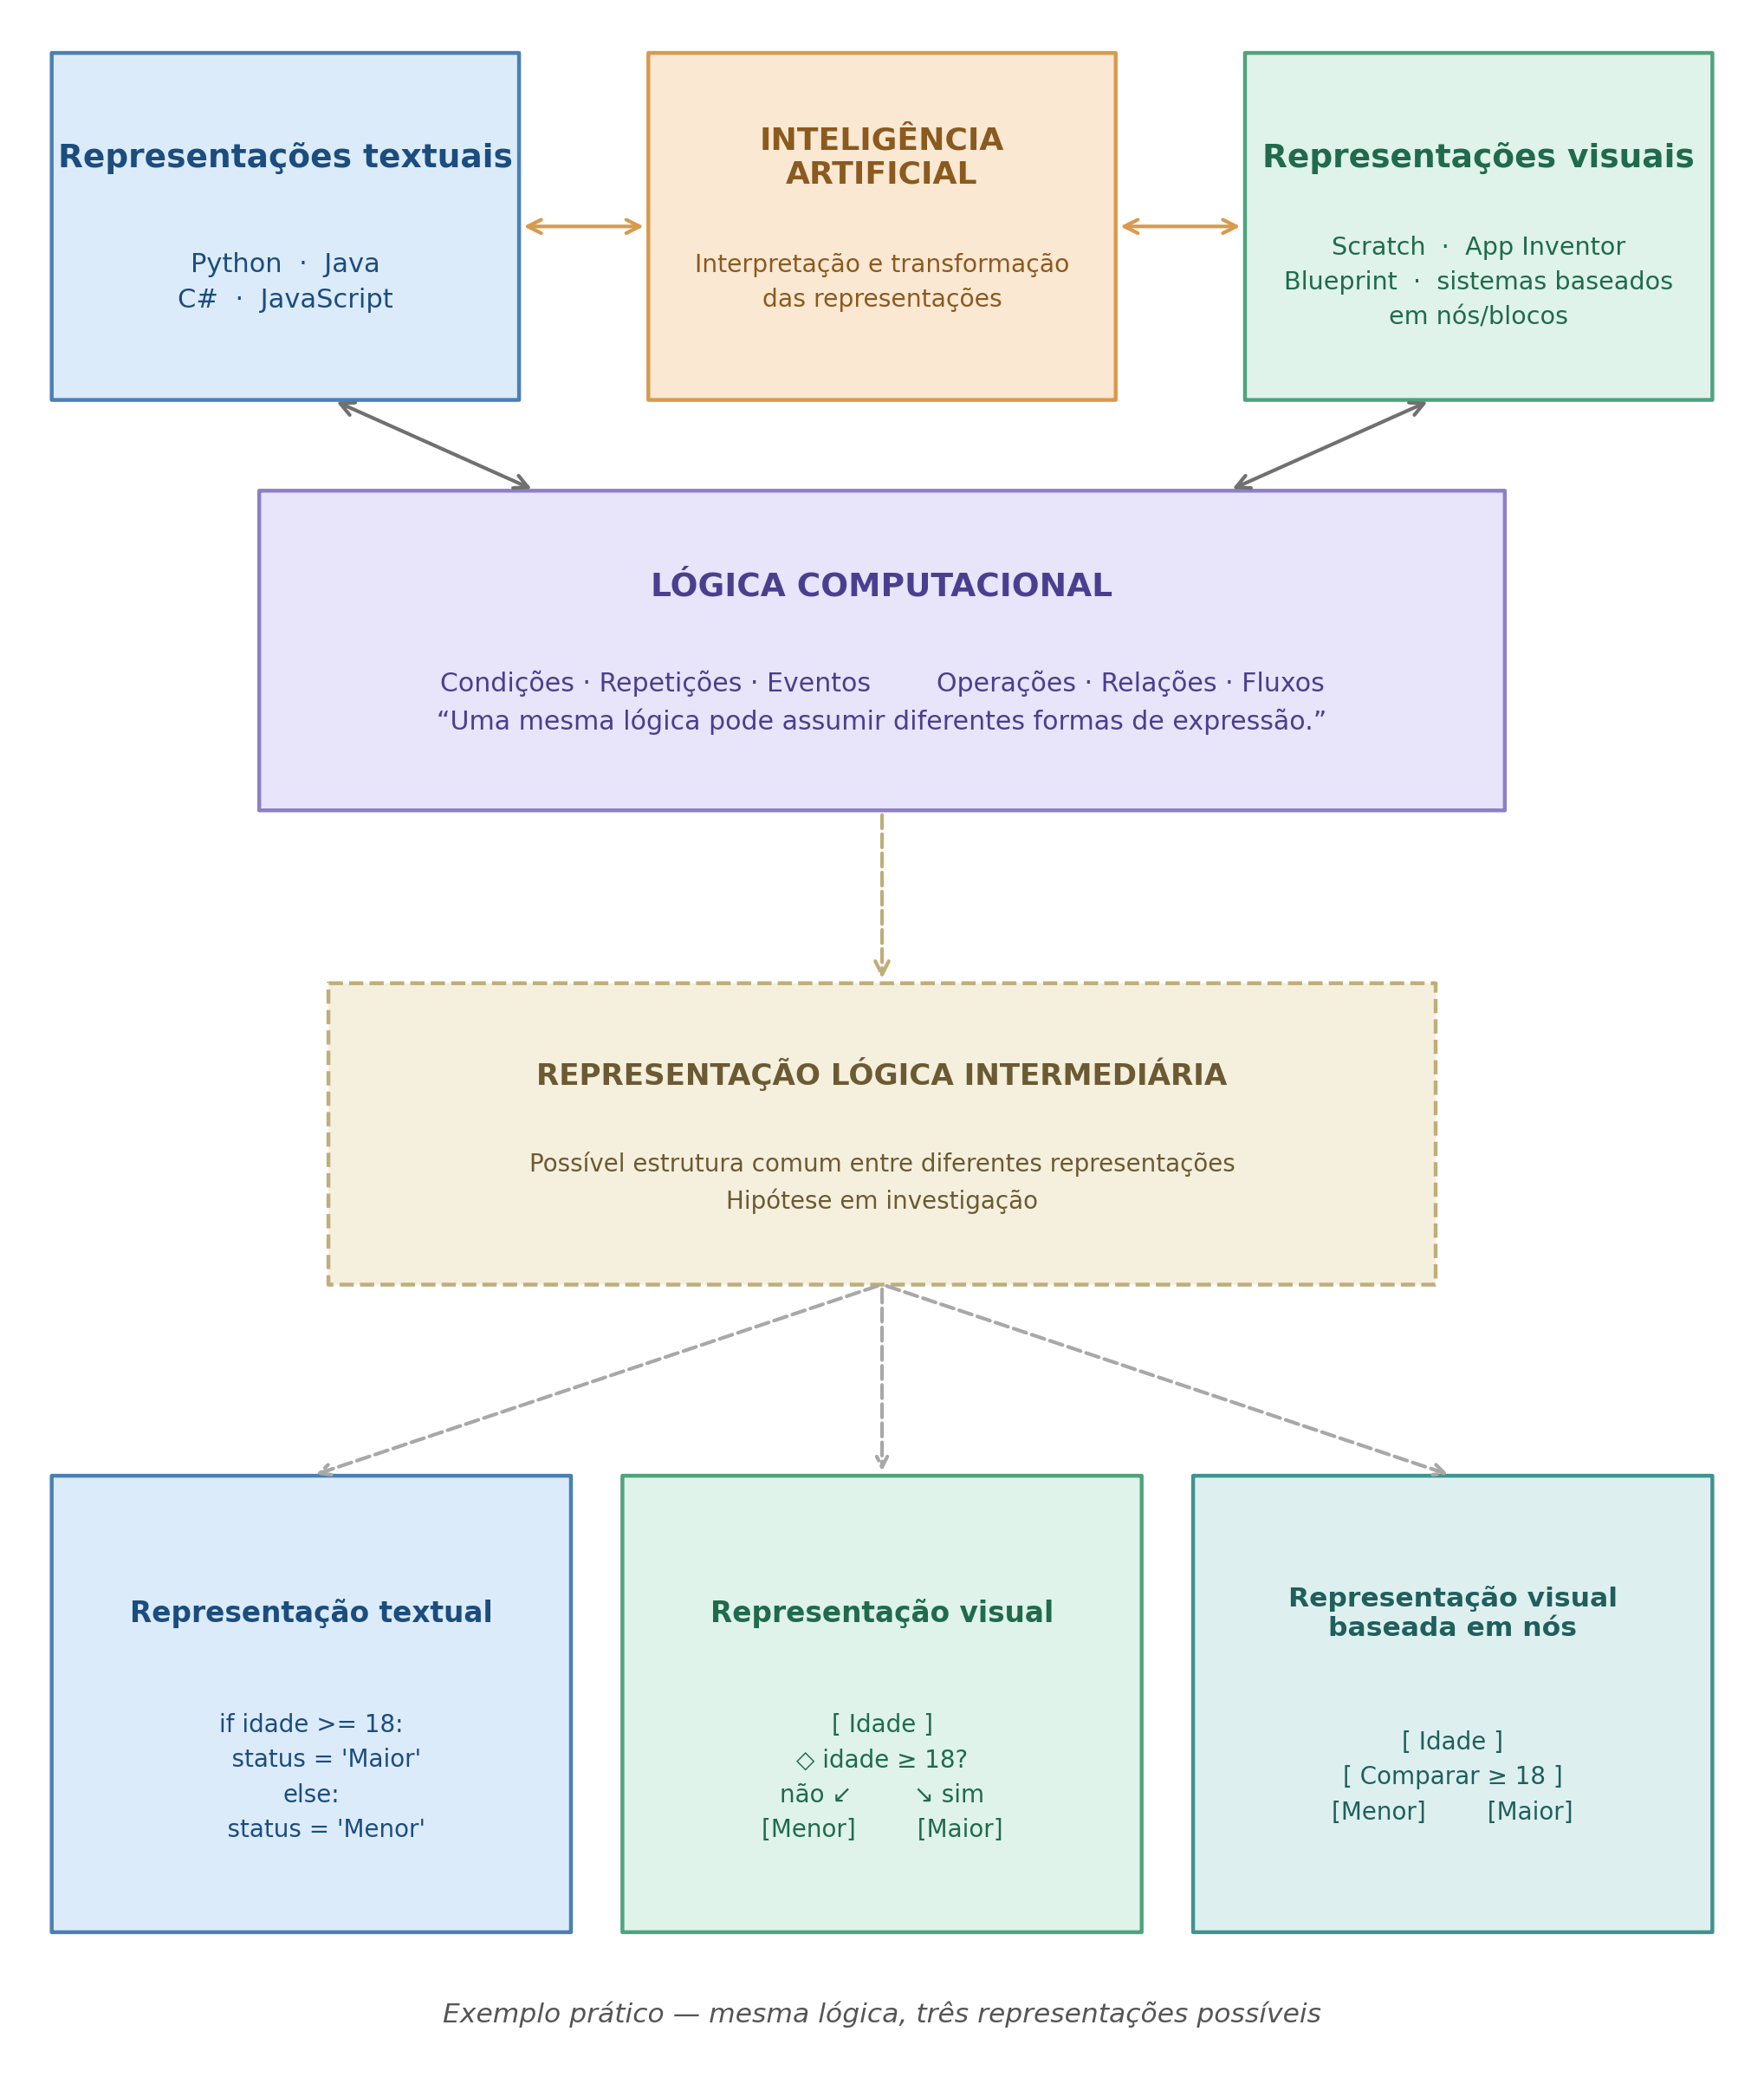
\includegraphics[width=\textwidth]{images/figura1_traducao_representacoes.png}
    \legend{Fonte: elaboração do autor com base em \citeonline{abelson1996} e \citeonline{myers1990}.}
    \label{fig:figura1_traducao_representacoes}
\end{figure}

\chapter{Desenvolvimento}
\section{Abstração e Representação da Lógica Computacional}

\subsection{O conceito de abstração em computação}

A abstração é considerada um dos conceitos fundamentais da Ciência da Computação, sendo utilizada para representar sistemas complexos por meio de modelos simplificados que destacam apenas os aspectos relevantes para determinado contexto. Segundo \citeonline{abelson1996}, a abstração permite que problemas computacionais sejam compreendidos e manipulados em diferentes níveis, reduzindo a necessidade de lidar diretamente com todos os detalhes de implementação, conforme a Figura \ref{fig:processo_abstracao}.

\begin{figure}[H]
    \centering
\caption{Processo de abstração aplicado à Ciência da Computação.}
    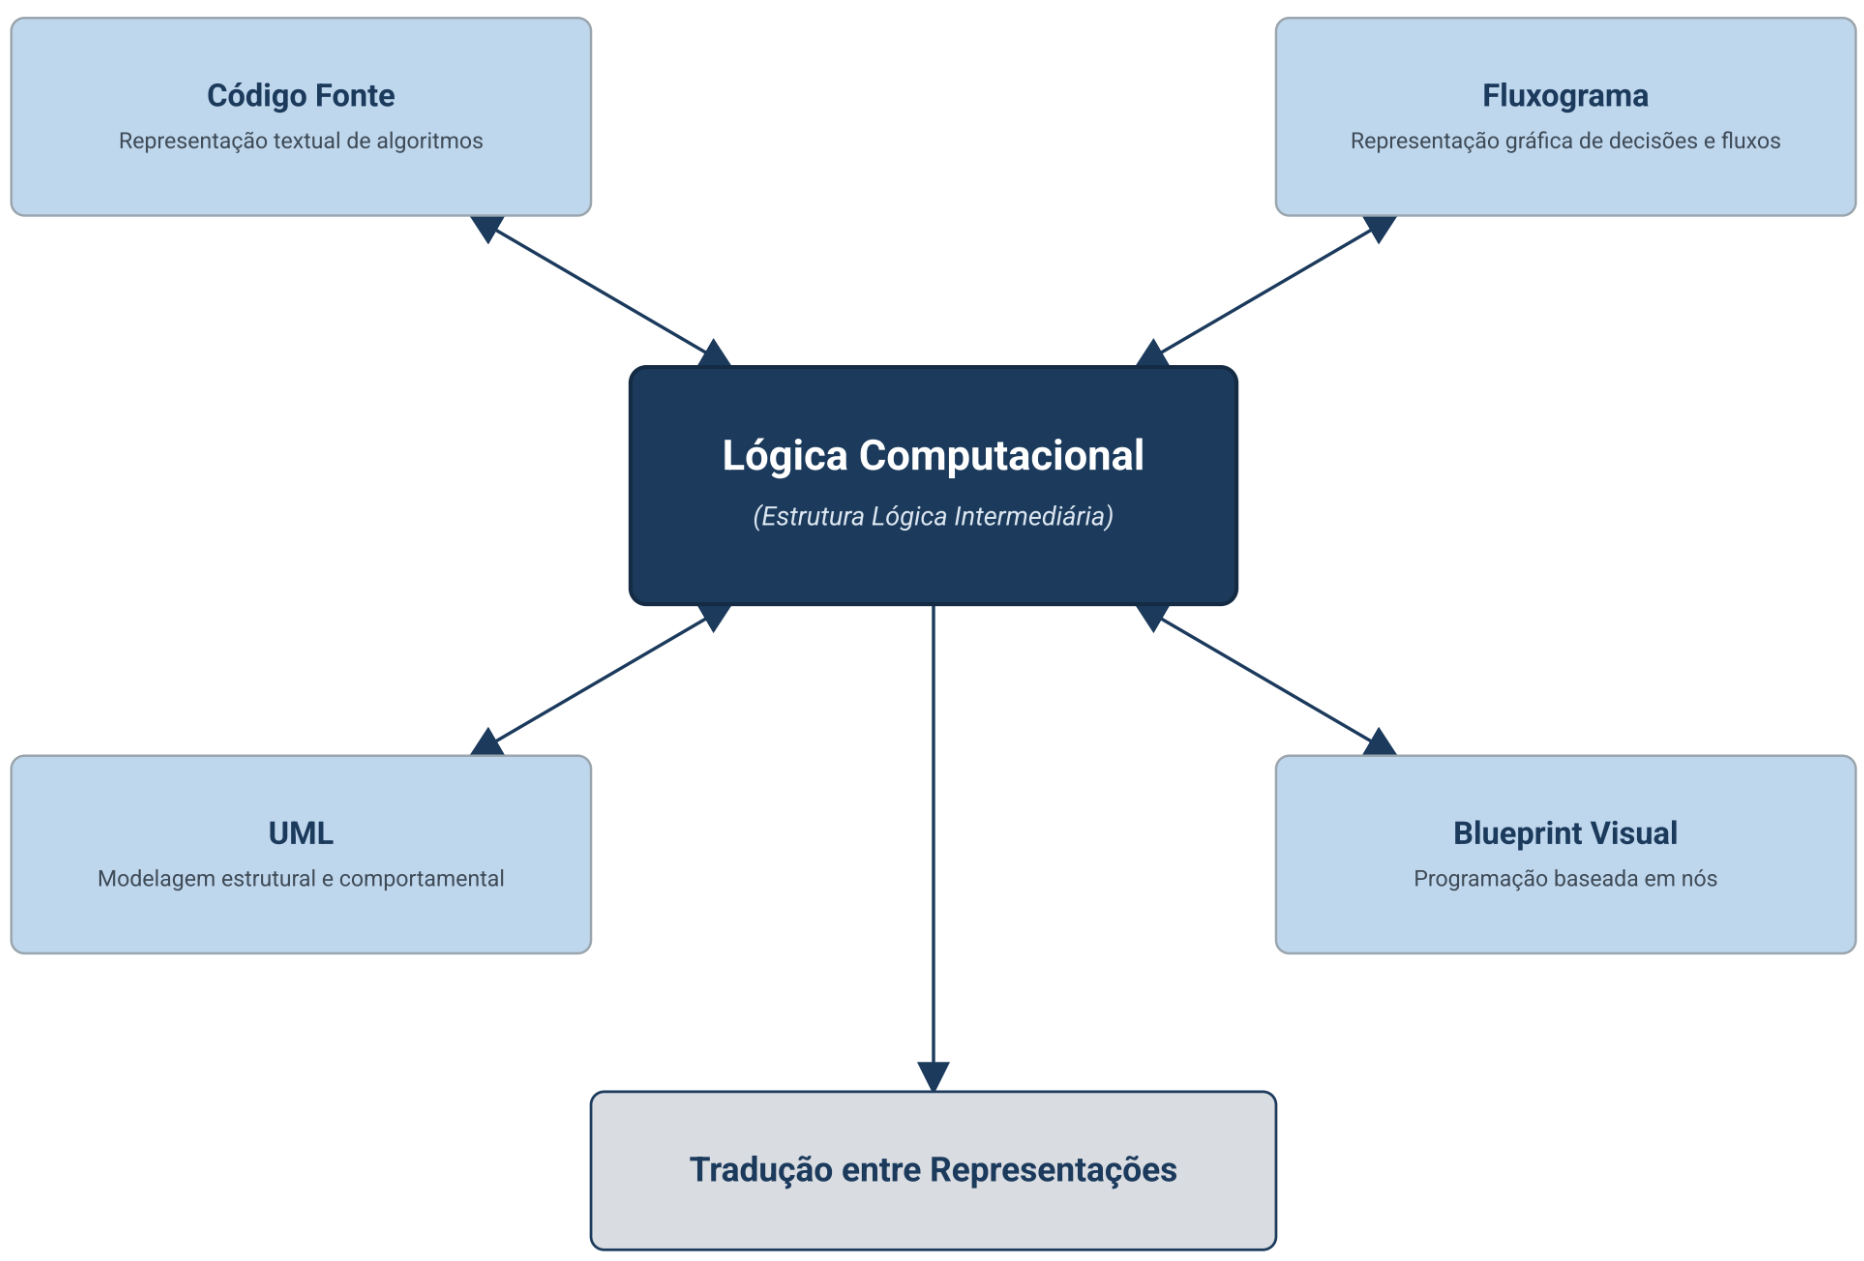
\includegraphics[width=\textwidth]{images/processo_abstracao.png}
\legend{Fonte: elaboração do autor com base em \citeonline{abelson1996}.}
    \label{fig:processo_abstracao}
\end{figure}


No desenvolvimento de software, a abstração está presente em diversas camadas, desde as linguagens de programação até as interfaces utilizadas pelos usuários finais. Cada camada oculta parte da complexidade da camada inferior, permitindo que desenvolvedores e usuários interajam com sistemas computacionais de maneira mais eficiente \cite{abelson1996}. Dessa forma, uma mesma lógica pode ser representada por diferentes mecanismos sem que seu significado fundamental seja alterado.

A compreensão desse conceito é especialmente relevante para esta pesquisa, uma vez que a hipótese investigada parte da possibilidade de que diferentes representações computacionais, como código textual e \textit{blueprints} visuais, possam expressar uma mesma estrutura lógica subjacente. Nesse contexto, a abstração torna-se um elemento central para compreender como a lógica computacional pode ser representada e interpretada em diferentes formatos.


\subsection{Lógica computacional independente da linguagem}

A lógica computacional pode ser compreendida como um conjunto de regras, decisões e processos que definem o comportamento de um sistema independentemente da linguagem utilizada para implementá-lo. Nesse contexto, as linguagens de programação atuam como mecanismos de representação dessa lógica, fornecendo estruturas sintáticas capazes de expressar algoritmos e comportamentos computacionais \cite{abelson1996}.

Segundo \citeonline{knuth1968}, os algoritmos constituem a base da computação, sendo independentes da tecnologia ou linguagem utilizada para sua implementação. Dessa forma, uma mesma solução lógica pode ser representada em diferentes linguagens de programação sem que seu objetivo fundamental seja alterado. O que muda é a forma de representação, enquanto a lógica subjacente permanece preservada.

Embora \citeonline{knuth1968} trate especialmente da independência entre algoritmos e linguagens textuais, esse mesmo princípio pode ser estendido às representações visuais. Uma decisão condicional, por exemplo, pode ser descrita por comandos em uma linguagem textual ou por elementos gráficos em fluxogramas e \textit{blueprints}, sem que a relação lógica entre a condição e seus possíveis fluxos de execução seja modificada. Dessa forma, a independência entre lógica e representação não se limita às linguagens de programação, estendendo-se também às formas visuais de representação computacional.

Essa independência entre lógica e representação, sustentada pelos conceitos de abstração de \citeonline{abelson1996} e pela noção de algoritmo de \citeonline{knuth1968}, constitui um dos fundamentos teóricos para investigar a viabilidade de traduções entre código textual e representações visuais. Compreender a lógica como uma estrutura separada de sua forma de representação é, portanto, condição necessária para analisar as relações existentes entre os diferentes modelos abordados nas seções seguintes.

\subsection{Representações da lógica computacional}

A lógica computacional pode ser expressa por diferentes modelos de representação, que variam conforme o contexto, o nível de abstração e os objetivos pretendidos. Ao longo da evolução da computação, essas formas foram desenvolvidas para atender a finalidades distintas, como facilitar a compreensão, documentar processos ou implementar sistemas executáveis.

Essas representações podem ser organizadas segundo diferentes critérios. Quanto à forma, distinguem-se as representações textuais (como o pseudocódigo e as linguagens de programação) das representações visuais (como os fluxogramas, os diagramas UML e os ambientes de programação baseados em nós). Quanto à finalidade, algumas representações possuem caráter essencialmente descritivo ou documental, voltado à compreensão e à comunicação de algoritmos, enquanto outras são executáveis, capazes de produzir diretamente o comportamento que descrevem. Apesar dessas diferenças, todas compartilham o objetivo comum de representar comportamentos, decisões e processos computacionais.

Essa diversidade de representações foi sistematizada por \citeonline{myers1990}, que propôs taxonomias para a programação visual e a visualização de programas, evidenciando que elementos gráficos podem representar relações e fluxos lógicos sem substituir a lógica computacional subjacente. Nessa perspectiva, a representação visual não se opõe ao código textual, mas oferece uma forma alternativa de expressar a mesma estrutura lógica.

A coexistência de múltiplas representações para uma mesma lógica sugere a existência de uma estrutura comum que as conecta. Compreender como cada modelo organiza e expressa algoritmos é, assim, um passo necessário para examinar as relações entre representações textuais e visuais, tema aprofundado na seção seguinte, dedicada à programação visual e aos ambientes baseados em fluxos.
\section{Programação Visual e Ambientes Baseados em Fluxos}

\subsection{Conceitos de programação visual}

A programação visual é uma abordagem de desenvolvimento na qual a lógica computacional é representada por elementos gráficos, como blocos, nós e conexões, em vez de ser expressa exclusivamente por código textual. Essa forma de representação busca tornar a construção e compreensão de sistemas mais intuitiva, permitindo que processos e comportamentos sejam visualizados de maneira direta.

Conforme \citeonline{myers1990}, ambientes de programação visual foram desenvolvidos para facilitar a interação com sistemas computacionais por meio de representações gráficas da lógica. Embora utilizem elementos visuais, esses ambientes continuam baseados nos mesmos princípios computacionais encontrados nas linguagens tradicionais de programação.

Essa característica revela um aspecto central da programação visual: por se apoiar nos mesmos princípios computacionais das linguagens textuais, ela demonstra que um mesmo comportamento pode ser implementado tanto por código quanto por fluxos visuais. Essa equivalência é o que torna os ambientes visuais especialmente relevantes para esta pesquisa, e as próximas subseções examinam suas principais manifestações --- os fluxogramas, os blueprints e as plataformas de baixo código.

\subsection{Fluxogramas e representação de algoritmos}

Os fluxogramas constituem uma das formas mais tradicionais de representação visual de algoritmos. Por meio de símbolos padronizados e conexões direcionais, eles permitem representar decisões, processos e fluxos de execução de maneira gráfica, facilitando a compreensão da lógica computacional.

Além de sua função representativa, os fluxogramas são amplamente utilizados para documentar e comunicar algoritmos durante o desenvolvimento de software. Sua estrutura visual torna mais acessível a compreensão do comportamento de sistemas computacionais, especialmente em etapas de análise, planejamento e documentação.

Cabe destacar, no entanto, que os fluxogramas possuem caráter essencialmente descritivo. Eles representam a lógica de um algoritmo para fins de compreensão e comunicação, mas não constituem, por si sós, um mecanismo de execução: a lógica representada precisa ser posteriormente traduzida em código para ser executada por um sistema computacional. Essa distinção entre representar e executar é relevante para esta pesquisa, pois diferencia os fluxogramas de outras representações visuais, como os blueprints, capazes de executar diretamente a lógica que descrevem, conforme discutido na seção seguinte.


A Figura \ref{fig:logica_central_codigo_fluxograma} apresenta a lógica computacional como elemento central entre diferentes formas de representação. Nesse contexto, tanto o código-fonte quanto os fluxogramas podem expressar uma mesma estrutura lógica, diferenciando-se apenas pela forma como essa informação é apresentada ao desenvolvedor.

\begin{figure}[H]
    \centering
    \caption{Relação entre diferentes formas de representação da lógica computacional.}
    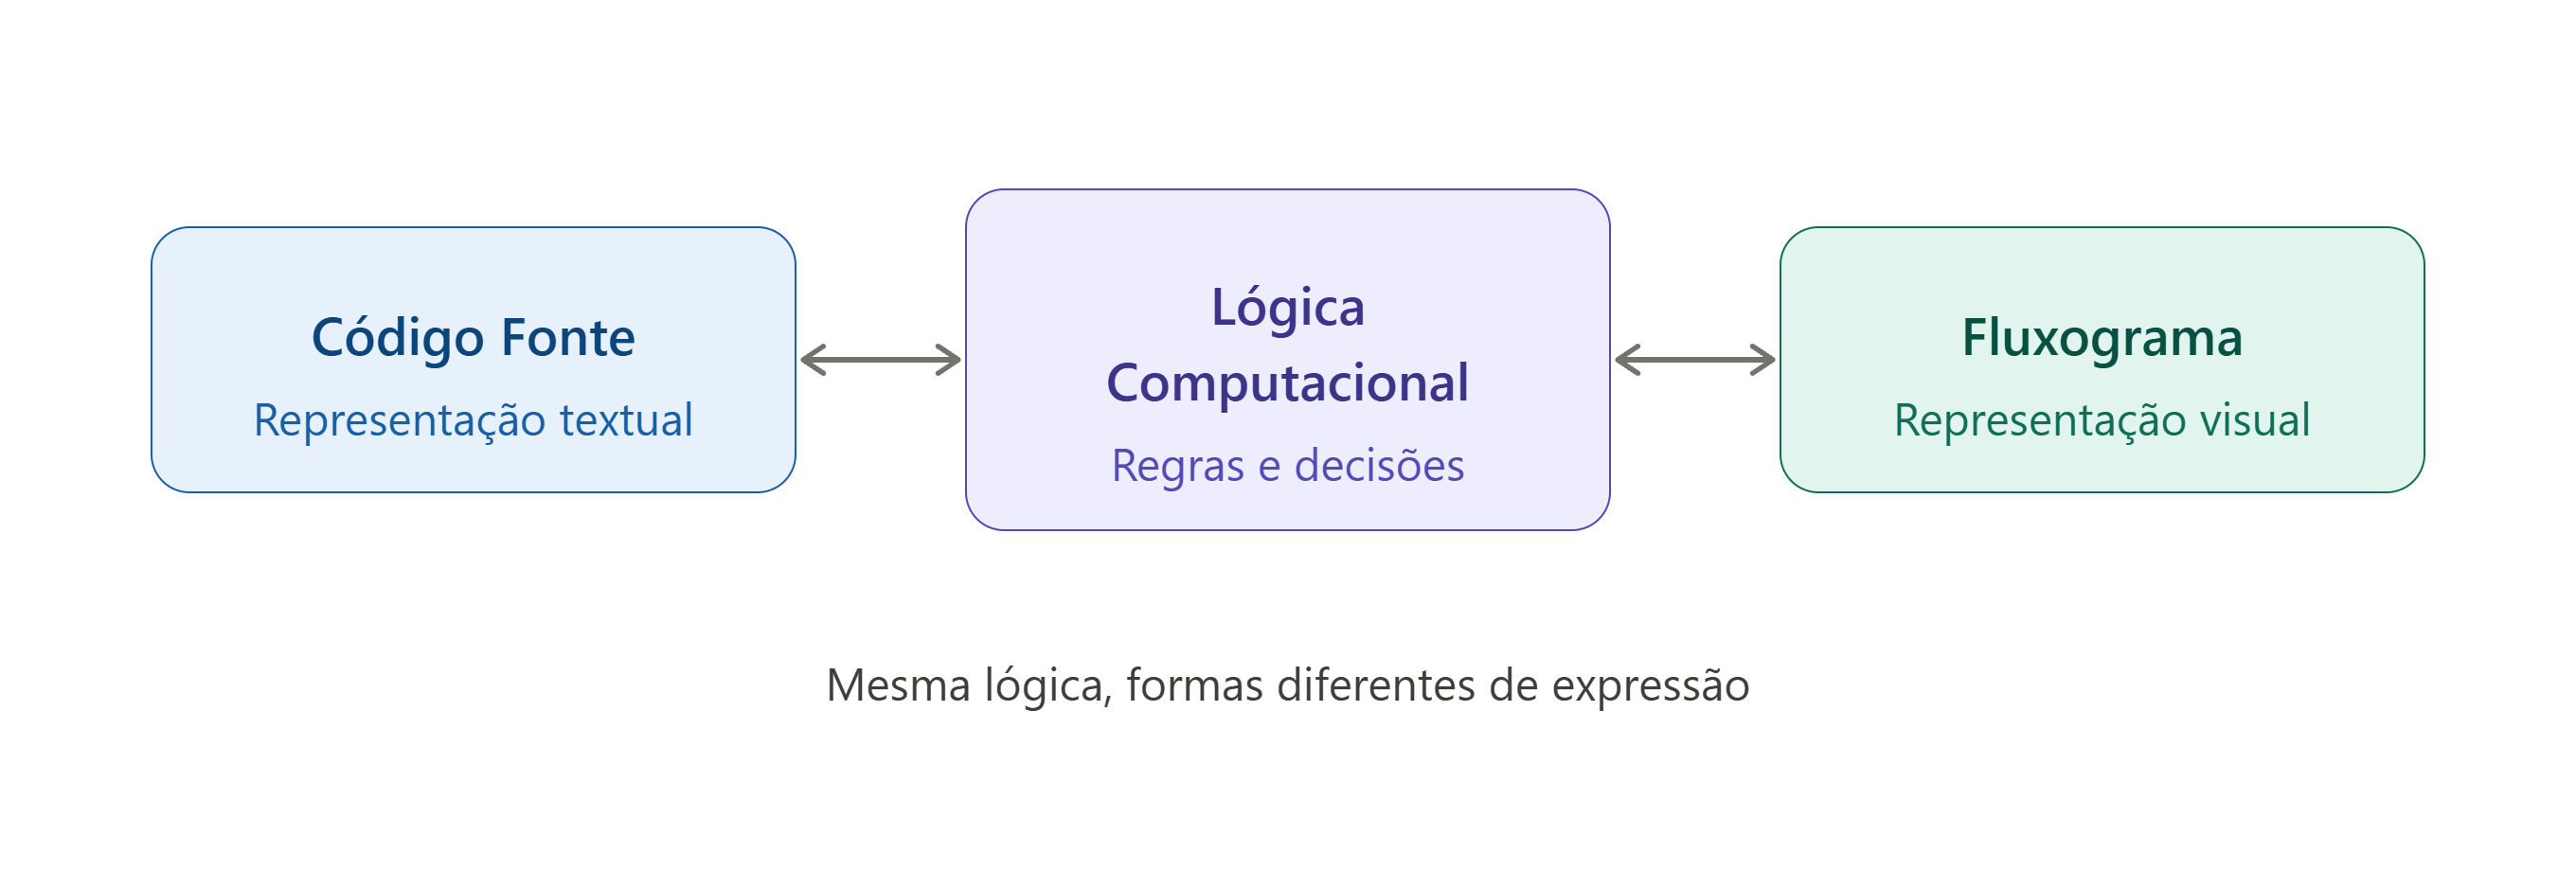
\includegraphics[width=0.85\textwidth]{images/logica_central_codigo_fluxograma.png}
    \legend{Fonte: elaboração do autor com base em \citeonline{abelson1996} e \citeonline{knuth1968}.}
    \label{fig:logica_central_codigo_fluxograma}
\end{figure}

\subsection{Blueprints e sistemas baseados em nós}

Os \textit{blueprints} e sistemas baseados em nós representam uma evolução dos modelos tradicionais de programação visual \cite{romero2014blueprint}. Nesses ambientes, a lógica computacional é construída por meio da conexão entre elementos gráficos denominados nós, que representam operações, eventos, decisões ou fluxos de dados.

Diferentemente dos fluxogramas, que possuem principalmente função descritiva e documental, os sistemas baseados em nós permitem a execução direta da lógica construída visualmente. Dessa forma, o fluxo visual deixa de ser apenas uma representação e passa a atuar como mecanismo efetivo de desenvolvimento de software.

Um dos exemplos mais conhecidos dessa abordagem é o sistema Blueprint da Unreal Engine, utilizado para o desenvolvimento de jogos e aplicações interativas. Nesse ambiente, programadores e designers podem construir comportamentos complexos por meio da conexão visual de nós, reduzindo a necessidade de escrita manual de código textual.

Essa característica reforça a hipótese de que a lógica computacional pode ser separada de sua forma de representação. Embora os \textit{blueprints} utilizem elementos visuais, os comportamentos implementados seguem os mesmos princípios algorítmicos encontrados nas linguagens de programação tradicionais.

A documentação oficial da Epic Games \cite{epic_blueprint} descreve o sistema Blueprint como uma interface de scripting visual que disponibiliza recursos de programação por meio de nós conectados. A solidez lógica dessa abordagem é evidenciada por trabalhos que demonstram ser possível aplicar verificação formal sobre scripts construídos em blueprints. \citeonline{wayama2022blueprint}, por exemplo, aplicaram model checking a programas desenvolvidos no Blueprint da Unreal Engine 5, evidenciando que a lógica representada visualmente pode ser formalmente analisada. Isso reforça a ideia central desta pesquisa: a de que a representação visual expressa uma estrutura lógica computacional bem definida, e não apenas um recurso gráfico de apoio.

Nesse contexto, os sistemas baseados em nós demonstram que diferentes formas de representação podem expressar uma mesma estrutura lógica, aspecto que se relaciona diretamente com a proposta desta pesquisa. A Figura \ref{fig:blueprint_if_idade} ilustra esse conceito por meio do mesmo exemplo lógico apresentado na Figura \ref{fig:figura1_traducao_representacoes} --- a condição \texttt{if idade >= 18} ---, desta vez expressa no formato de nós conectados característico dos sistemas blueprint. Embora a representação seja visualmente distinta do código textual e do fluxograma, o comportamento lógico subjacente permanece idêntico.

\begin{figure}[H]
    \centering
    \caption{Exemplo de lógica computacional representada por meio de um sistema visual baseado em nós (blueprint).}
    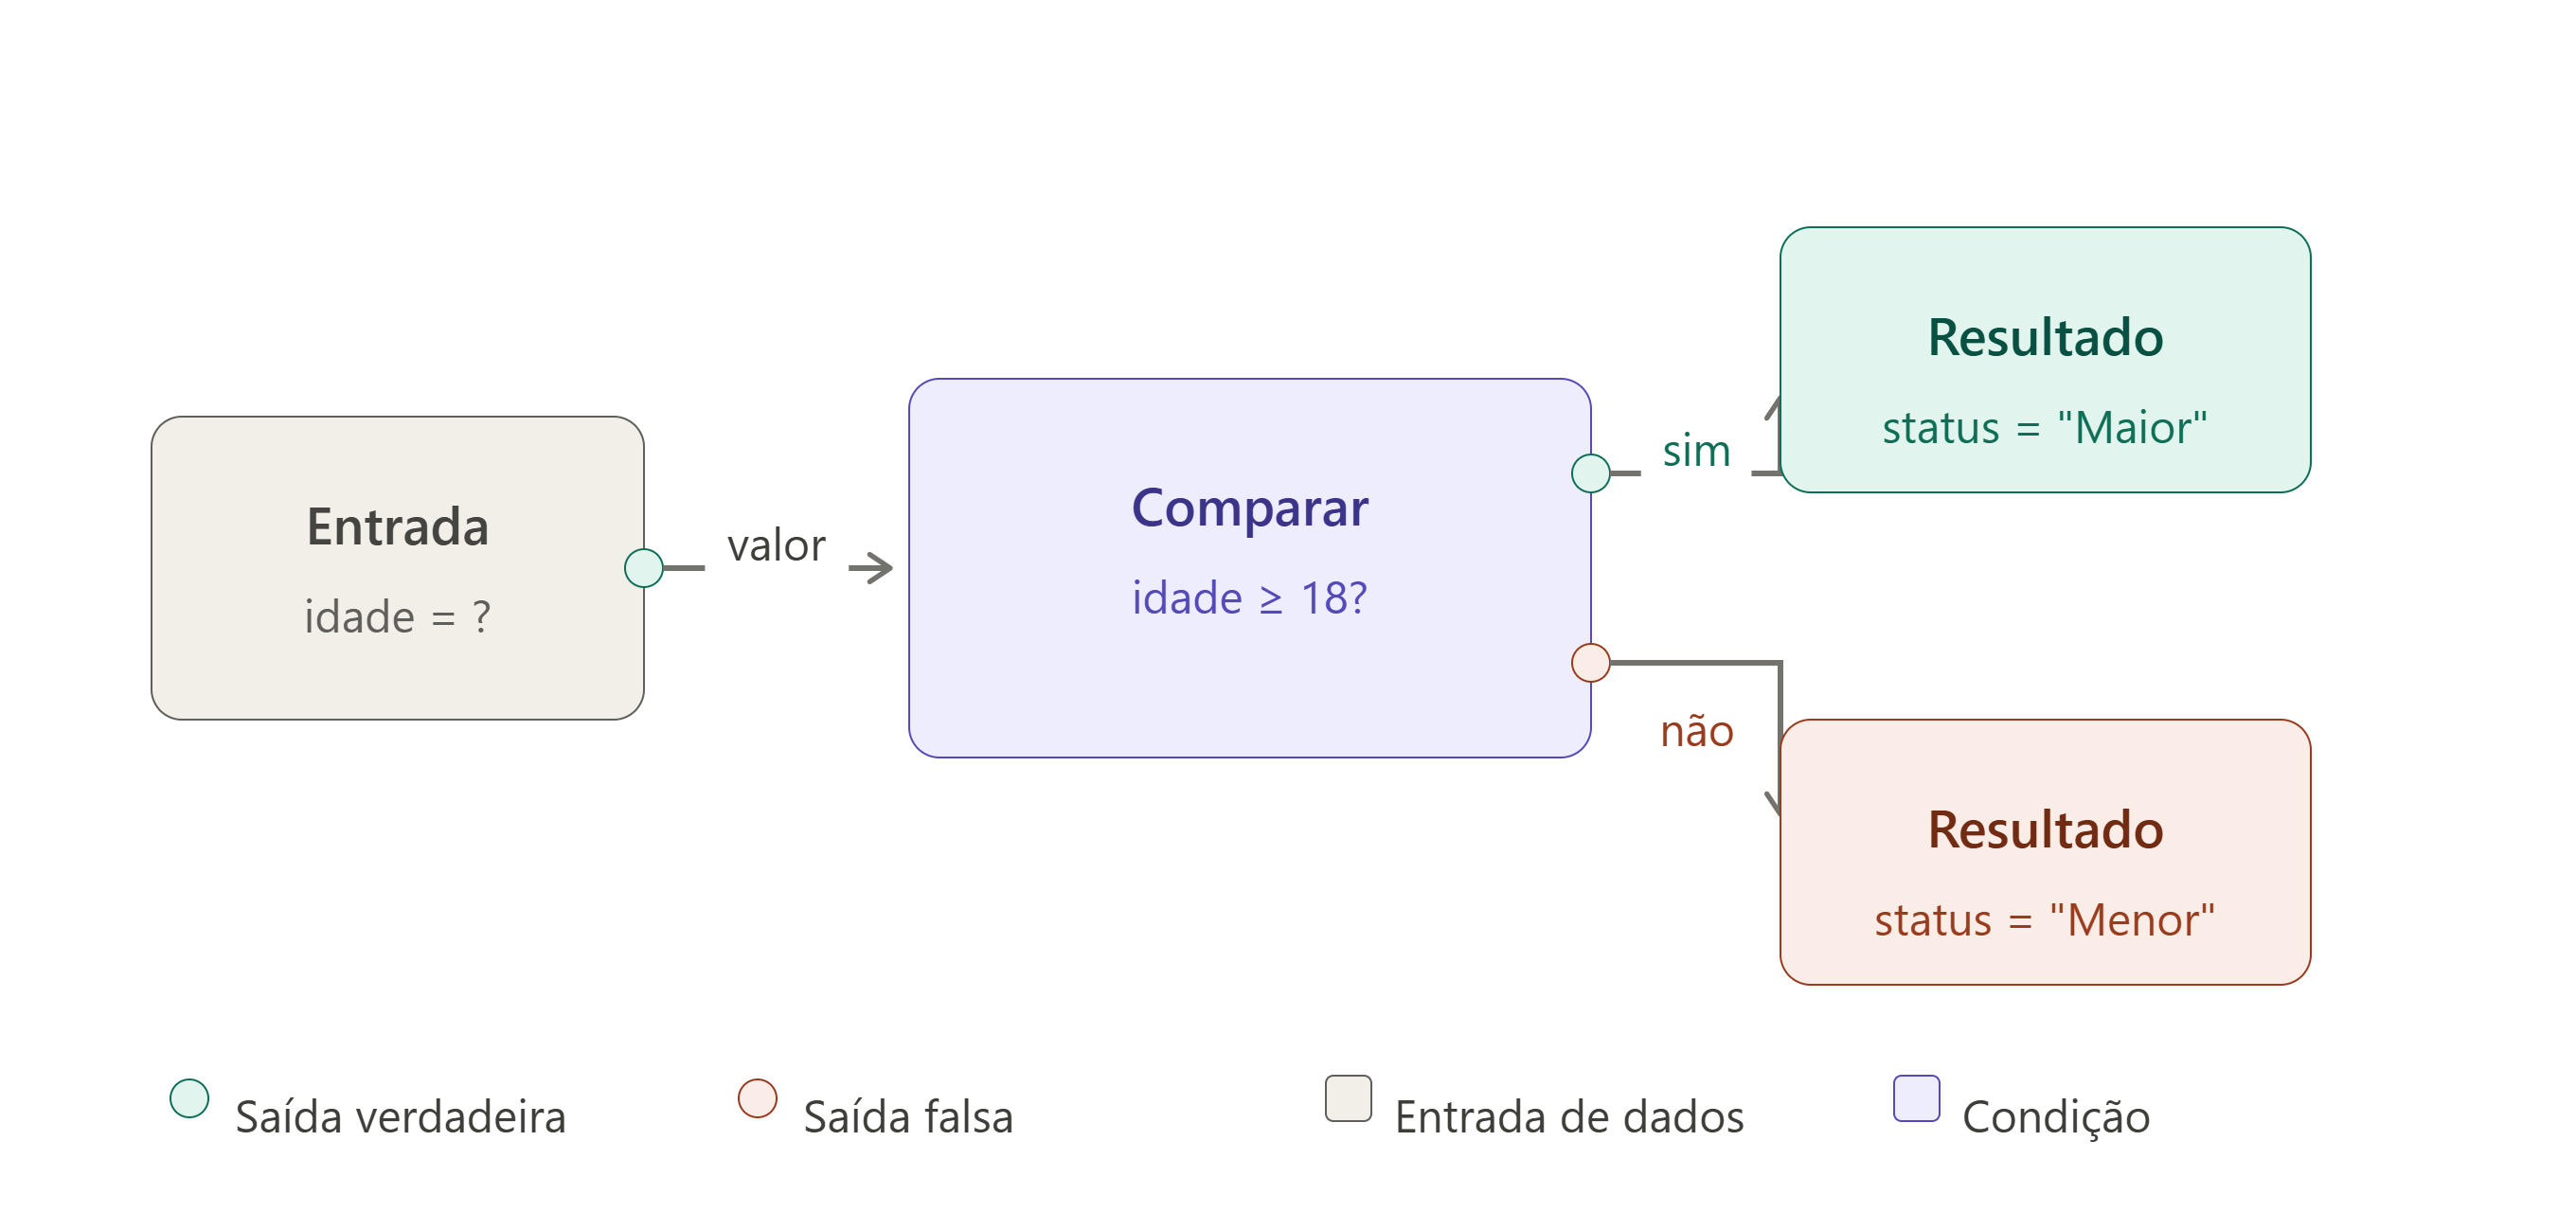
\includegraphics[width=\textwidth]{images/blueprint_if_idade.png}
    \legend{Fonte: elaboração do autor com base em \citeonline{romero2014blueprint} e \citeonline{epic_blueprint}.}
    \label{fig:blueprint_if_idade}
\end{figure}

\subsection{Plataformas Low-Code e No-Code}

As plataformas \textit{Low-Code} e \textit{No-Code} surgiram como uma evolução dos ambientes de programação visual, buscando reduzir a complexidade do desenvolvimento de software por meio de interfaces gráficas e componentes reutilizáveis. Nessas plataformas, grande parte da lógica é construída por meio da conexão entre blocos, fluxos e elementos visuais, diminuindo a necessidade de escrita manual de código.

A utilização de representações visuais para construção de sistemas computacionais contribui para ampliar a acessibilidade ao desenvolvimento de software, permitindo que usuários com diferentes níveis de conhecimento técnico participem da criação de soluções digitais \cite{myers1990}.

Nesse contexto, plataformas como \textit{n8n}, \textit{Node-RED}, \textit{Microsoft Power Automate} e outras ferramentas de automação utilizam fluxos visuais para representar processos, integrações e comportamentos computacionais. Embora apresentem interfaces simplificadas, essas plataformas continuam baseadas nos mesmos princípios lógicos encontrados nas linguagens tradicionais de programação \cite{silva2023lowcode}.

Cada uma dessas ferramentas adota uma forma própria de representar a lógica, ainda que compartilhem o princípio comum dos fluxos visuais. No \textit{n8n}, a lógica é organizada em nós que atuam como blocos de construção de um fluxo de trabalho, responsáveis por iniciar a execução, buscar e enviar dados e manipular informações \cite{n8ndocs}. O \textit{Node-RED}, por sua vez, baseia-se na programação orientada a eventos e no encadeamento de nós, sendo amplamente aplicado à integração de dispositivos e à Internet das Coisas \cite{nodereddocs}. Já o \textit{Microsoft Power Automate} estrutura a lógica em fluxos compostos por gatilhos, que iniciam a execução a partir de um evento, e ações, que definem as operações realizadas em seguida \cite{powerautomatedocs}. Apesar das diferenças visuais e estruturais entre essas representações, todas expressam decisões, condições e sequências de execução, evidenciando que uma mesma lógica computacional pode assumir formas distintas conforme o ambiente utilizado.


\subsubsection*{Síntese da seção}

A análise dos ambientes apresentados demonstra que a lógica computacional pode ser representada por diferentes modelos visuais (fluxogramas, blueprints e plataformas \textit{Low-Code} ou \textit{No-Code}) sem perder sua capacidade de expressar algoritmos, decisões e fluxos de execução. Embora cada abordagem possua características e objetivos distintos, todas compartilham um princípio comum: a utilização de elementos visuais para representar estruturas lógicas, sem alteração de seu significado fundamental.

Essa constatação fornece suporte teórico à hipótese investigada nesta pesquisa e estabelece a base para o capítulo seguinte, no qual se discute como essa estrutura lógica comum pode atuar como elemento intermediário na tradução entre diferentes representações computacionais.

\chapter{Proposta Conceitual da Pesquisa}
\section{O problema da tradução entre representações computacionais}

Conforme discutido nos capítulos anteriores, uma mesma lógica computacional pode ser expressa por diferentes representações, como linguagens textuais, fluxogramas, \textit{blueprints} e plataformas \textit{Low-Code} ou \textit{No-Code}, todas capazes de descrever decisões, condições e fluxos de execução.

O problema central abordado por esta pesquisa está no fato de que essas representações são desenvolvidas e utilizadas como ambientes isolados entre si. Cada ferramenta define sua própria sintaxe, sua própria semântica e seu próprio modo de construir a lógica, sem mecanismos que permitam transitar de uma representação para outra. Na prática, uma lógica construída em um ambiente não pode ser reaproveitada em outro: para migrar de uma representação textual para uma visual, ou vice-versa, é necessário reconstruí-la manualmente desde o início.

Essa ausência de comunicação entre representações gera retrabalho, dificulta a colaboração entre perfis técnicos distintos e impede que o conhecimento expresso em uma forma seja transferido diretamente para outra. Diante disso, coloca-se a questão que motiva esta proposta: seria possível identificar uma estrutura lógica comum a essas representações, capaz de servir de base para converter uma na outra sem perda de significado computacional? É essa questão que as seções seguintes buscam responder.

\section{Lógica computacional como estrutura intermediária}

A resposta que esta pesquisa propõe para a questão levantada anteriormente é que essa estrutura comum é a própria lógica computacional, compreendida de forma independente da representação que a expressa. Embora linguagens de programação, fluxogramas, \textit{blueprints} e plataformas \textit{Low-Code} ou \textit{No-Code} apresentem diferenças visuais e sintáticas, todas descrevem os mesmos elementos fundamentais: decisões, condições, operações, eventos e sequências de execução.

A proposta é tratar esses elementos fundamentais como uma camada situada entre a lógica e suas diferentes formas de representação. Nessa camada, a lógica deixa de estar presa à sintaxe de uma linguagem ou ao formato gráfico de uma ferramenta e passa a ser descrita de forma abstrata: uma condição é apenas uma condição, com seus possíveis desfechos, e uma sequência de operações é apenas uma ordem de execução, sem depender de como cada ambiente a desenha ou escreve. É essa descrição abstrata, despida da forma, que constitui a estrutura lógica intermediária.

Essa ideia apoia-se no conceito de abstração discutido no Capítulo 2 \cite{abelson1996}. Da mesma forma que uma linguagem de alto nível oculta detalhes de implementação sem alterar o comportamento do programa, a estrutura lógica intermediária oculta as particularidades de cada representação, preservando apenas aquilo que define o comportamento computacional. Assim, fluxogramas, \textit{blueprints} e código textual passam a ser vistos como diferentes projeções de uma mesma estrutura.

Compreender a lógica dessa forma é o que torna a tradução entre representações conceitualmente possível. Se duas representações podem ser reduzidas à mesma estrutura intermediária, é possível interpretar uma delas, identificar sua estrutura lógica e, a partir dela, gerar a outra, sem perda do comportamento originalmente definido.

Um exemplo simples ilustra esse princípio. A decisão de verificar se uma idade é maior ou igual a 18 pode ser escrita em código como uma estrutura \texttt{if/else}, desenhada em um fluxograma como um losango de decisão com dois caminhos, ou montada em um \textit{blueprint} como um nó de comparação com duas saídas. As três formas têm aparência completamente diferente, mas descrevem a mesma estrutura intermediária: uma condição com dois desfechos possíveis. O que muda é a forma; a lógica permanece a mesma.

A Figura \ref{fig:estrutura_intermediaria} resume essa ideia, posicionando a lógica computacional como substrato comum a partir do qual as diferentes representações podem ser interpretadas.
\begin{figure}[H]
    \centering
    \caption{Representação conceitual da lógica computacional como estrutura intermediária entre diferentes formas de representação computacional.}
    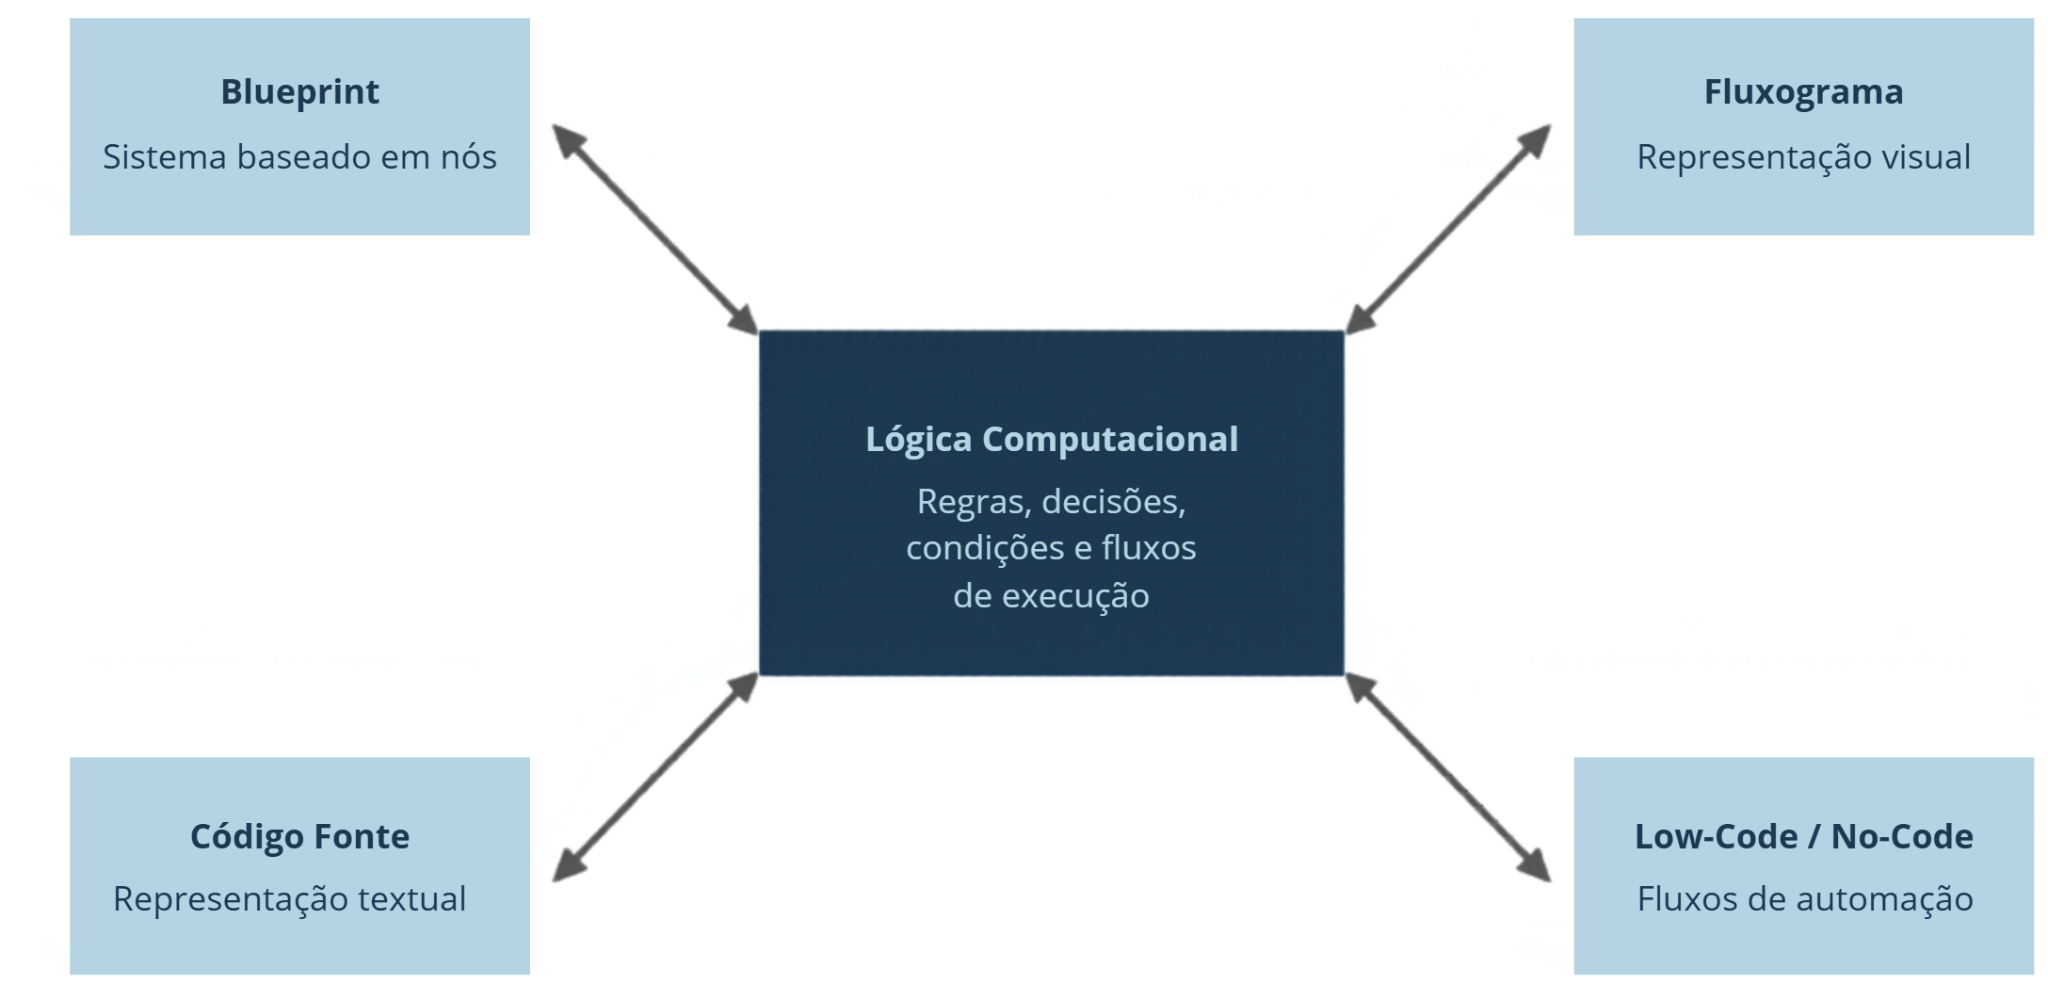
\includegraphics[width=\textwidth]{images/estrutura_intermediaria.png}
    \legend{Fonte: elaboração do autor com base em \citeonline{abelson1996} e \citeonline{myers1990}.}
    \label{fig:estrutura_intermediaria}
\end{figure}

\section{Modelo conceitual proposto}

Com base na hipótese desenvolvida na seção anterior, esta pesquisa propõe um modelo conceitual de conversão organizado em três etapas. Na primeira, uma representação de origem é interpretada, e sua lógica é extraída na forma da estrutura lógica intermediária. Na segunda, essa estrutura mantém a lógica de maneira abstrata, independente de qualquer linguagem ou ferramenta. Na terceira, a partir dessa estrutura, gera-se uma representação de destino, textual ou visual, preservando o comportamento originalmente definido.

O ponto central desse modelo é que a conversão nunca ocorre diretamente de uma representação para outra, mas sempre por meio da estrutura intermediária. Essa escolha não é apenas conceitual: converter cada representação diretamente em todas as demais exigiria um mecanismo específico para cada par de formatos, e a quantidade desses mecanismos cresceria rapidamente a cada nova representação incluída. Ao adotar uma estrutura intermediária comum, basta que cada representação saiba ser interpretada para essa estrutura e gerada a partir dela, reduzindo o problema a um conjunto menor e reaproveitável de etapas.

Para que isso seja possível, o modelo considera que elementos como condições, operações, eventos e sequências de execução podem ser identificados em qualquer representação e organizados nessa estrutura comum. São esses elementos, e não a aparência de cada ambiente, que o modelo preserva ao longo de todo o processo de conversão.

A Figura \ref{fig:modelo_conceitual} representa esse fluxo, no qual uma representação de origem é interpretada, convertida na estrutura lógica intermediária e, a partir dela, transformada em uma representação de destino.
\begin{figure}[H]
\centering
\caption{Modelo conceitual proposto para conversão entre representações computacionais.}
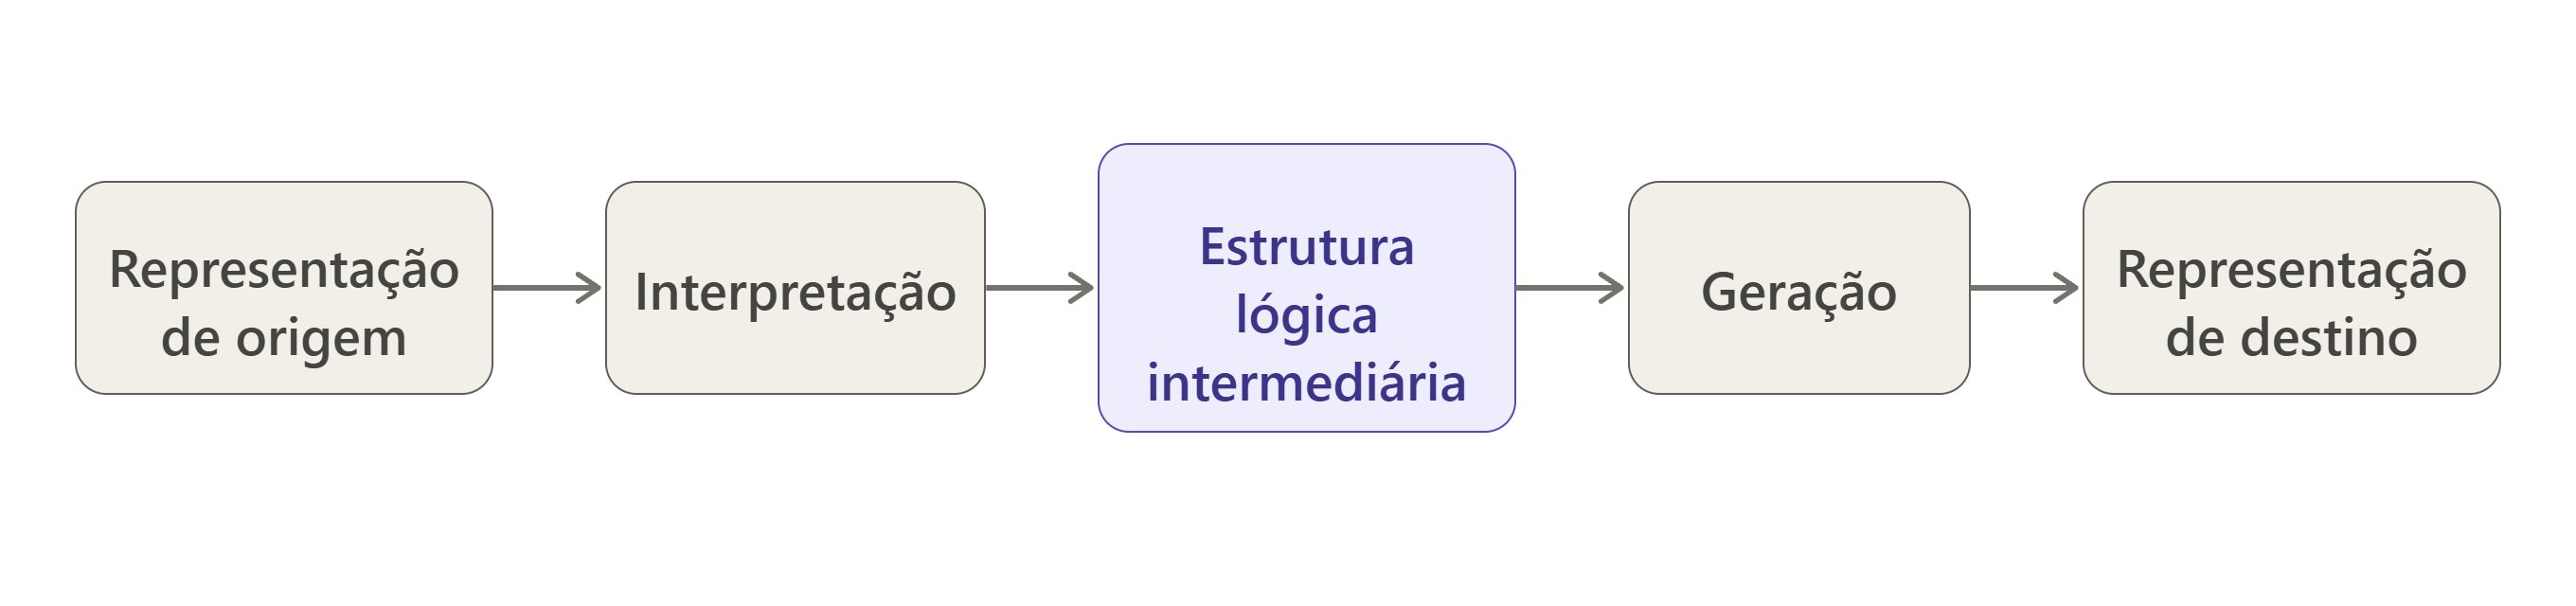
\includegraphics[width=\textwidth]{images/figura6_modelo_conceitual.png}
\legend{Fonte: elaboração do autor.}
\label{fig:modelo_conceitual}
\end{figure}



\section{Cenários de conversão entre representações}

Conforme antecipado na introdução, a inteligência artificial pode atuar como mecanismo de apoio nesse processo de conversão. Em vez de depender de regras fixas definidas manualmente para cada par de representações, um mecanismo assistido por IA poderia identificar a estrutura lógica subjacente a uma representação de origem e reconstruí-la em uma representação de destino. Dessa forma, a IA atuaria como uma camada responsável por interpretar, comparar e gerar representações computacionais, preservando o comportamento lógico originalmente definido.

Nesse contexto, um algoritmo descrito em código-fonte pode ser convertido para um fluxograma, assim como um fluxograma pode ser transformado em uma representação textual equivalente. O mesmo princípio pode ser aplicado a sistemas baseados em nós e plataformas \textit{Low-Code} ou \textit{No-Code}, desde que a lógica computacional subjacente seja preservada durante o processo de conversão. 

A Figura \ref{fig:arquitetura_camada_ia} apresenta a arquitetura conceitual do modelo, destacando o papel da IA como camada mediadora entre as representações e a estrutura lógica subjacente.

\begin{figure}[H]
\centering
\caption{Arquitetura conceitual da camada de IA como elemento mediador entre representações computacionais.}
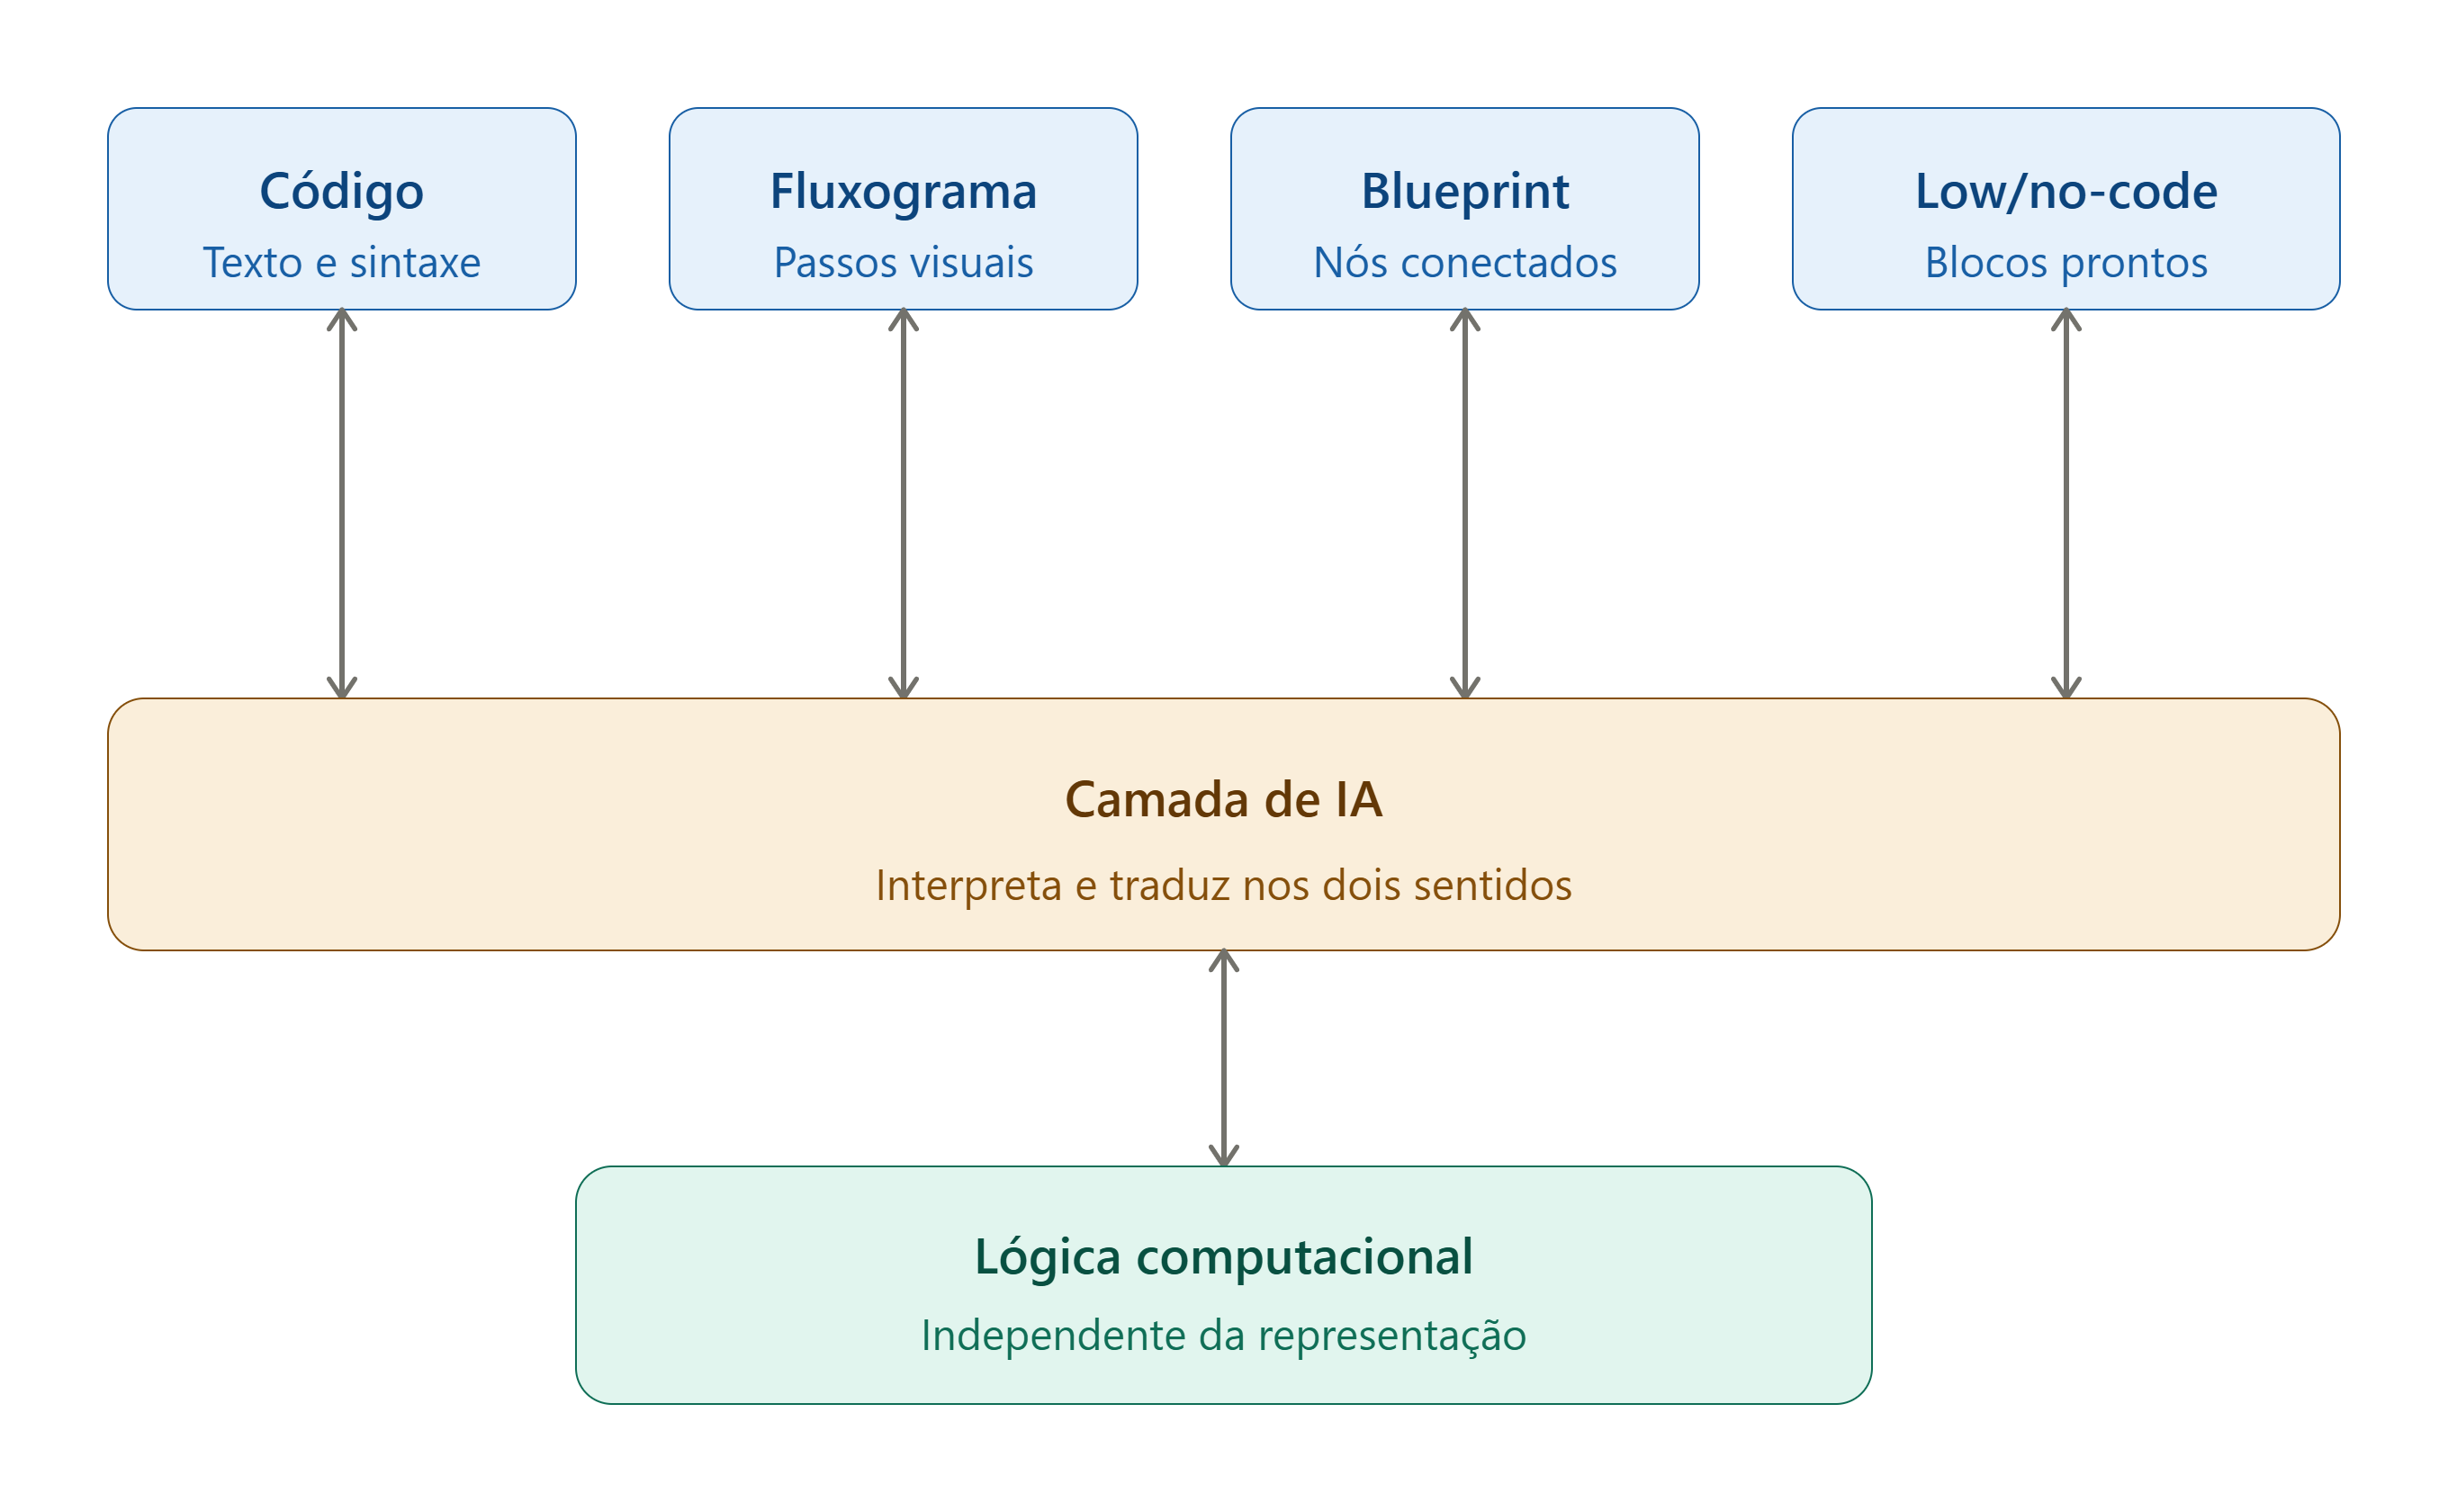
\includegraphics[width=\textwidth]{images/arquitetura_camada_ia.png}
\legend{Fonte: elaboração do autor.}
\label{fig:arquitetura_camada_ia}
\end{figure}

A partir dessa perspectiva, diferentes representações computacionais podem ser compreendidas como manifestações distintas de uma mesma lógica computacional. Dessa forma, a conversão entre código-fonte, fluxogramas, \textit{blueprints} e plataformas \textit{Low-Code} ou \textit{No-Code} \cite{silva2024lowcode} torna-se conceitualmente possível por meio da identificação de uma estrutura lógica intermediária, preservando o significado computacional originalmente definido.

\section{Limitações da proposta}

Esta pesquisa tem caráter conceitual e exploratório, conforme definido em sua metodologia. Por essa razão, não contempla o desenvolvimento de um sistema funcional de tradução nem a validação experimental do modelo: a precisão, a viabilidade e o desempenho de um mecanismo de conversão constituem uma etapa posterior, que pressupõe a base conceitual aqui estabelecida.

No plano técnico, há a diversidade entre os ambientes de desenvolvimento. Embora diferentes representações compartilhem princípios lógicos semelhantes, cada ferramenta possui sua própria sintaxe, semântica e forma de execução, e determinados recursos de uma representação podem não ter equivalente direto em outra. Esses casos delimitam até onde a tradução pode ser automática, indicando pontos em que mecanismos de adaptação seriam necessários.

O modelo concentra-se ainda na lógica interna de um algoritmo: suas decisões, condições e fluxos de execução. Aspectos que extrapolam essa lógica, como dependências de serviços externos ou a coordenação entre componentes distribuídos, não fazem parte do escopo desta proposta. Delimitar a análise à estrutura lógica é uma escolha deliberada, que permite isolar o problema central da pesquisa.

Apesar dessas limitações, a proposta oferece uma contribuição própria: um modelo conceitual que trata a lógica computacional como elemento separável de sua forma de representação, fornecendo uma base teórica para a tradução entre representações distintas. A partir dessa base, a implementação e a validação prática apresentam-se como continuidade natural desta pesquisa.

\chapter{Considerações Finais}
Esta pesquisa teve como objetivo investigar se diferentes representações computacionais (linguagens textuais, fluxogramas, \textit{blueprints} e plataformas \textit{Low-Code} e \textit{No-Code}) compartilham uma estrutura lógica comum capaz de servir de base para a tradução entre elas. Por meio de revisão bibliográfica e análise conceitual, esse objetivo foi alcançado: o trabalho identificou e caracterizou diferentes formas de representação e demonstrou, no plano teórico, a relação lógica que as une.

Verificou-se que, apesar de suas diferenças visuais e sintáticas, essas representações descrevem os mesmos elementos lógicos (decisões, condições, operações e sequências de execução), o que confirma a hipótese de que a lógica computacional pode ser compreendida de forma independente da forma que a expressa.

A principal contribuição do trabalho é o modelo conceitual proposto, no qual a lógica computacional atua como estrutura intermediária entre representações: uma representação de origem é interpretada, sua lógica é organizada nessa estrutura comum e, a partir dela, uma nova representação é gerada. O modelo reúne, sob uma mesma base teórica, representações que costumam ser tratadas como ambientes isolados.

Esse resultado tem implicações relevantes. Ao mostrar que código e representações visuais são formas distintas de uma mesma lógica, e não realidades incompatíveis, a pesquisa oferece uma base para repensar a interoperabilidade entre ambientes de desenvolvimento, favorecer a comunicação entre perfis técnicos distintos e aproximar os modelos textuais e visuais de construção de software.

Como continuidade natural, a validação prática do modelo e o desenvolvimento de mecanismos automáticos de conversão permitiriam avaliar empiricamente a abordagem e estendê-la a cenários mais complexos. Ainda assim, ao demonstrar a consistência teórica da separação entre lógica e representação, esta pesquisa oferece uma base sólida para futuras investigações sobre tradução e interoperabilidade entre representações computacionais.
    

% --------------------------------------
% REFERÊNCIAS
% --------------------------------------
% Colocar SUAS referências no arquivo TCC.bib
% Pode ser criada com o BibDesk - https://bibdesk.sourceforge.io/
% Ou manualmente seguindo o arquivo que deixei como modelo
% --------------------------------------
\bibliography{TCC}

\end{document}
